% Aberdeen style guide should be followed when using this
% layout. Their template powerpoint slide is used to extract the
% Aberdeen color and logo but is otherwise ignored (it has little or
% no formatting in it anyway).
%
% http://www.abdn.ac.uk/documents/style-guide.pdf

%%%%%%%%%%%%%%%%%%%% Document Class Settings %%%%%%%%%%%%%%%%%%%%%%%%%
% Pick if you want slides, or draft slides (no animations)
%%%%%%%%%%%%%%%%%%%%%%%%%%%%%%%%%%%%%%%%%%%%%%%%%%%%%%%%%%%%%%%%%%%%%%
%Normal document mode
\documentclass[10pt,compress]{beamer}
%%%%%Draft or handout mode
%\documentclass[10pt,compress,handout]{beamer}
%\documentclass[10pt,compress,handout,ignorenonframetext]{beamer}

%%%%%%%%%%%%%%%%%%%% General Document settings %%%%%%%%%%%%%%%%%%%%%%%
% These settings must be set for each presentation
%%%%%%%%%%%%%%%%%%%%%%%%%%%%%%%%%%%%%%%%%%%%%%%%%%%%%%%%%%%%%%%%%%%%%%
\newcommand{\shortname}{Dr Jeff Gomes}
\newcommand{\fullname}{Dr Jeff Gomes}
\institute{School of Engineering}
\newcommand{\emailaddress}{jefferson.gomes@abdn.ac.uk}
\newcommand{\logoimage}{../FigBanner/UoAHorizBanner}
\title{Engineering Thermodynamics (EG3521)}
\subtitle{Module 2: Production of Power from Heat}
\date[18-24/02/2014]{18-24 February 2014}


%%%%%%%%%%%%%%%%%%%% Template settings %%%%%%%%%%%%%%%%%%%%%%%%%%%%%%%
% You shouldn't have to change below this line, unless you want to.
%%%%%%%%%%%%%%%%%%%%%%%%%%%%%%%%%%%%%%%%%%%%%%%%%%%%%%%%%%%%%%%%%%%%%%
\usecolortheme{whale}
\useoutertheme{infolines}

% Use the fading effect for items that are covered on the current
% slide.
\beamertemplatetransparentcovered

% We abuse the author command to place all of the slide information on
% the title page.
\author[\shortname]{%
  \fullname\\\ttfamily{\emailaddress}
}


%At the start of every section, put a slide indicating the contents of the current section.
%\AtBeginSection[] {
%  \begin{frame}
%    \frametitle{Section Outline}
%    \tableofcontents[currentsection]
%  \end{frame}
%}

% Allow the inclusion of movies into the Presentation! At present,
% only the Okular program is capable of playing the movies *IN* the
% presentation.
\usepackage{multimedia}
\usepackage{animate}

% \usepackage[usenames,dvipsnames]{pstricks}
% \usepackage{epsfig}
% \usepackage{pst-grad} % For gradients
% \usepackage{pst-plot} % For axes


%%%%% Color settings
\usepackage{color}
%% The background color for code listings (i.e. example programs)
\definecolor{lbcolor}{rgb}{0.9,0.9,0.9}%
\definecolor{UoARed}{rgb}{0.64706, 0.0, 0.12941}
\definecolor{UoALight}{rgb}{0.85, 0.85, 0.85}
\definecolor{UoALighter}{rgb}{0.92, 0.92, 0.92}
\setbeamercolor{structure}{fg=UoARed} % General background and higlight color
\setbeamercolor{frametitle}{bg=black} % General color
\setbeamercolor{frametitle right}{bg=black} % General color
\setbeamercolor{block body}{bg=UoALighter} % For blocks
\setbeamercolor{structure}{bg=UoALight} % For blocks
% Rounded boxes for blocks
\setbeamertemplate{blocks}[rounded]

%%%%% Font settings
% Aberdeen requires the use of Arial in slides. We can use the
% Helvetica font as its widely available like so
% \usepackage{helvet}
% \renewcommand{\familydefault}{\sfdefault}
% But beamer already uses a sans font, so we will stick with that.

% The size of the font used for the code listings.
\newcommand{\goodsize}{\fontsize{6}{7}\selectfont}

% Extra math packages, symbols and colors. If you're using Latex you
% must be using it for formatting the math!
\usepackage{amscd,amssymb} \usepackage{amsfonts}
\usepackage[mathscr]{eucal} \usepackage{mathrsfs}
\usepackage{latexsym} \usepackage{amsmath} \usepackage{bm}
\usepackage{amsthm} \usepackage{textcomp} \usepackage{eurosym}
% This package provides \cancel{a} and \cancelto{a}{b} to "cancel"
% expressions in math.
\usepackage{cancel}

% Get rid of font warnings as modern LaTaX installations have scalable
% fonts
\usepackage{type1cm} 

%\usepackage{enumitem} % continuous numbering throughout enumerate commands

% For exact placement of images/text on the cover page
\usepackage[absolute]{textpos}
\setlength{\TPHorizModule}{1mm}%sets the textpos unit
\setlength{\TPVertModule}{\TPHorizModule} 

% Source code formatting package
\usepackage{listings}%
\lstset{ backgroundcolor=\color{lbcolor}, tabsize=4,
  numberstyle=\tiny, rulecolor=, language=C++, basicstyle=\goodsize,
  upquote=true, aboveskip={1.5\baselineskip}, columns=fixed,
  showstringspaces=false, extendedchars=true, breaklines=false,
  prebreak = \raisebox{0ex}[0ex][0ex]{\ensuremath{\hookleftarrow}},
  frame=single, showtabs=false, showspaces=false,
  showstringspaces=false, identifierstyle=\ttfamily,
  keywordstyle=\color[rgb]{0,0,1},
  commentstyle=\color[rgb]{0.133,0.545,0.133},
  stringstyle=\color[rgb]{0.627,0.126,0.941}}

% Allows the inclusion of other PDF's into the final PDF. Great for
% attaching tutorial sheets etc.
\usepackage{pdfpages}
\setbeamercolor{background canvas}{bg=}  

% Remove foot note horizontal rules, they occupy too much space on the slide
\renewcommand{\footnoterule}{}

% Force the driver to fix the colors on PDF's which include mixed
% colorspaces and transparency.
\pdfpageattr {/Group << /S /Transparency /I true /CS /DeviceRGB>>}

% Include a graphics, reserve space for it but
% show it on the next frame.
% Parameters:
% #1 Which slide you want it on
% #2 Previous slides
% #3 Options to \includegraphics (optional)
% #4 Name of graphic
\newcommand{\reserveandshow}[4]{%
\phantom{\includegraphics<#2|handout:0>[#3]{#4}}%
\includegraphics<#1>[#3]{#4}%
}

\begin{document}

% Title page layout
\begin{frame}
  \titlepage
  \vfill%
  \begin{center}
    \includegraphics[clip,width=0.8\textwidth]{\logoimage}
  \end{center}
\end{frame}

% Table of contents
%\frame{ \frametitle{Slides Outline}
%  \tableofcontents
%}


%%%%%%%%%%%%%%%%%%%% The Presentation Proper %%%%%%%%%%%%%%%%%%%%%%%%%
% Fill below this line with \begin{frame} commands! It's best to
% always add the fragile option incase you're going to use the
% verbatim environment.
%%%%%%%%%%%%%%%%%%%%%%%%%%%%%%%%%%%%%%%%%%%%%%%%%%%%%%%%%%%%%%%%%%%%%%

\section{Module 2.2: Introduction of Gas Power Systems}

%%%
%%% Slide
%%%
\subsection{Motivation}
\begin{frame}
 \frametitle{Aims and Objectives}
 At the end of this set of lectures, you should be able to:
 \begin{enumerate}[(i)]
  \item <1-> Assess the performance of gas power cycles;
  \item <2-> Solve problems based on the Brayton, Otto, Diesel, Stirling and Ericsson cycles;
  \item <3-> Perform second-law analysis of gas power cycles and;
  \item <4-> Identify simplifying assumptions for second-law analysis of gas power cycles.
  %\item <5-> 
 \end{enumerate}
\end{frame}
%%%
%%% Slide
%%%
\subsection{Motivation}
\begin{frame}
 \frametitle{Outline of Lectures}
 \begin{enumerate}[(i)]
  \item <1-> Air Standard Efficiency
  \item <2-> Reciprocating Engines
  \item <3-> Ideal Carnot Cycle
  \item <4-> Otto Cycle (Constant Volume)
  \item <5-> Diesel Cycle (Constant Pressure)
  \item <6-> Dual Combustion Cycle
  \item <7-> Comparison of Otto, Diesel and Dual Combustion Cycles
  \item <8-> Atkinson Cycle
  \item <9-> Ericsson Cycle
  \item <10-> Brayton Cycle (Gas Turbine)
 \end{enumerate}
\end{frame}
 
%%%
%%% Slide
%%%
\subsection{Bibliography} 
\begin{frame}
 \frametitle{Suggested References}
  Literature relevant for this module:
  \begin{enumerate}[(a)]
   \item J.M. Smith, H.C. Van Ness, M.M. Abbott, $\lq$Introduction to Chemical Engineering Thermodynamics', 6$^{th}$ Edition: Chapter 8;
   \item  M.J. Moran, H.N. Saphiro, D.D. Boettner, M.B. Bailey, $\lq$Principles of Engineering Thermodynamics',  7$^{th}$ Edition: Chapter 9;
   %\item A.B. Pippard, $\lq$Elements of Classical Thermodynamics' (1966): Chapters 2, 3 and 4;
   \item I. Muller, W.H. Muller, $\lq$Fundamentals of Thermodynamics and Applications', Chapter 3;
   \item \href{http://www.learnthermo.com}{http://www.learnthermo.com}, Chapter 9.
  \end{enumerate}
\end{frame}



\subsection{Air Standard Efficiency}
%%%
%%% Slide
%%%
\begin{frame}
 \frametitle{General Assumptions:}
  \begin{enumerate}
   \item <1-> In the first part of this Module we reviewed the definition of \textcolor{blue}{cycles} in which fuel is $\lq$burned' in a \textcolor{blue}{combustion chamber} with air, resulting in a stream of combustion products, i.e.;
   %\item <2-> In Module 2, we will focus on the thermochemical process called \textcolor{blue}{Combustion}, thus in this module we assume that no chemical reaction occurs in the cylinder
   \item <2-> Here, due to the complexity on thermodynamics analysis of gas power cycle, we will assume that \textcolor{blue}{air is the only work fluid} with an external heat source;
   \item <3-> Air behaves as an ideal gas with contant heat capacities at room  temperature $\left(MW=29\;g/gmol,\;C_{p}=1.005\;kJ/(kg.K),\;\text{and }C_{v}=0.718\;kJ/(kg.K)\right)$;
   \item <4-> Compression and expansion processes are adiabatic and with no internal friction;
   \item <5-> Exhausted process is replaced by a heat-rejection process that restores the working fluid to its initial state;
   \item <6-> Cycles in which the above is applied are called \textcolor{blue}{Air-Standard Cycle}.
  \end{enumerate}
\end{frame}

%%%
%%% Slide
%%%
\begin{frame}
 \frametitle{Air Standard Efficiency}
  \begin{enumerate}
   \item The efficiency of an engine using air as the working medium is called \textcolor{blue}{air standard efficiency} or \textcolor{blue}{ideal efficiency};
   \item In order to compare ideal and actual/real efficiencies, we introduce the relative efficiency:
    \begin{displaymath}
      \textcolor{blue}{\eta_{\text{relative}}=\displaystyle\frac{\text{Actual Thermal Efficiency}}{\text{Air-Standard Efficiency}}}
    \end{displaymath}
  \end{enumerate}
\end{frame}


\subsection{Reciprocating Engine}
%%%
%%% Slide
%%%
\begin{frame}
 \frametitle{Nomenclature}
 \begin{columns}
  \begin{column}[c]{0.4\linewidth}
   \begin{itemize}
    \item <1-> Bottom dead center (BDC): position of the piston in which the volume becomes \textcolor{blue}{maximum};
    \item <2-> Top dead center (TDC): position of the piston in which the volume becomes \textcolor{blue}{minimum} (i.e., clearance volume);
    \item <3-> Stroke: the largest distance that the piston can travel $\Longrightarrow$ $X_{\text{TDC}}-X_{\text{BDC}}$;
    \item <4-> Bore: diameter of the piston.
   \end{itemize}
  \end{column}
  \begin{column}[c]{0.6\linewidth}
   \begin{figure}%
    \begin{center}
     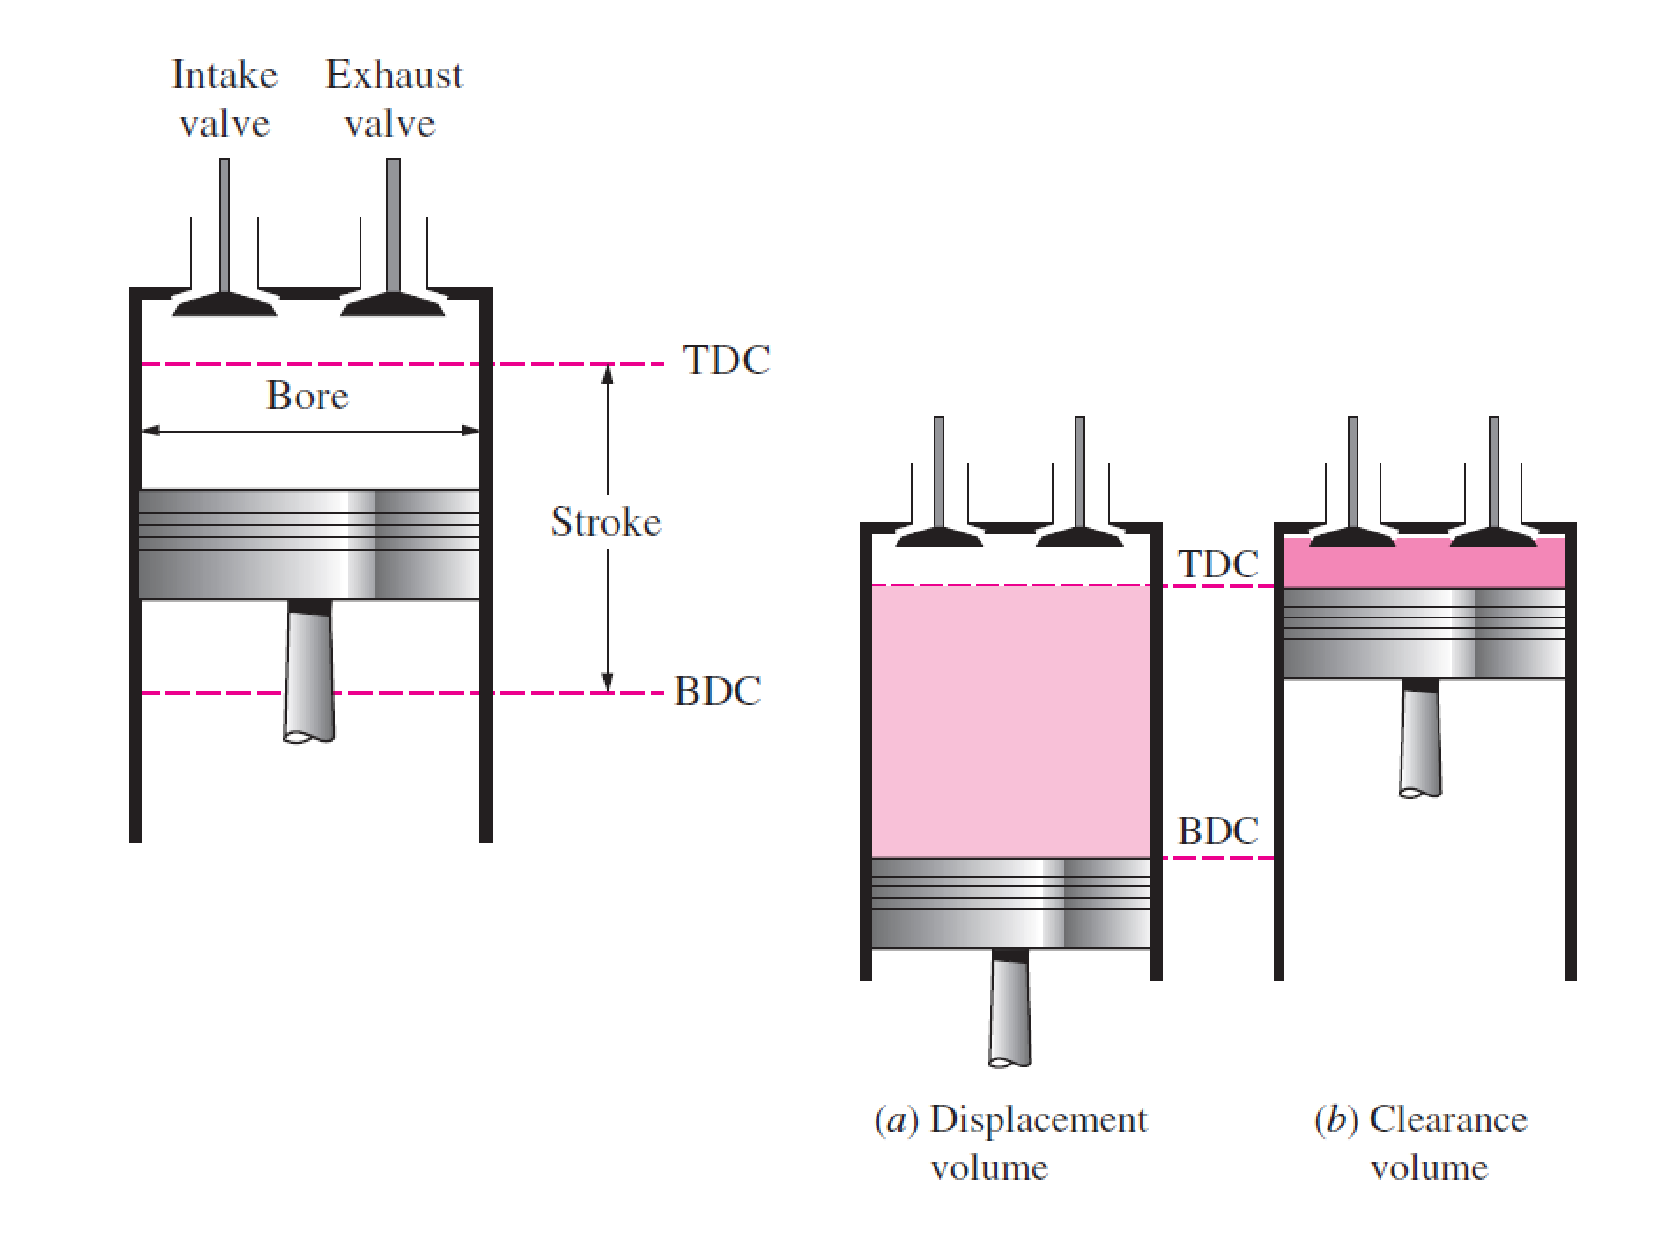
\includegraphics[width=7.5cm,clip]{./Pics/GasCycle_ReciprocatingEngine}
    \end{center}
   \end{figure}  
  \end{column}  
 \end{columns}
\end{frame}


%%%
%%% Slide
%%%
\begin{frame}
 \frametitle{Nomenclature}
 \begin{columns}
  \begin{column}[c]{0.4\linewidth}
   \begin{itemize}
    \item <1-> The Intake Valve is responsible to control the inflow of the air-fuel solution into the cylinder;
    \item <2-> The Exhaust Valve lets the combustion gases leave the cylinder;
    \item <3-> Displacement Volume: volume of the cylinder limited by $X_{\text{TDC}}$ and $X_{\text{BDC}}$ 
    \item <4-> Compression Ratio: $r=V_{\text{max}}/V_{\text{min}}=$ $V_{\text{BDC}}/V_{\text{TDC}}$ 
   \end{itemize}
  \end{column}
  \begin{column}[c]{0.6\linewidth}
   \begin{figure}%
    \begin{center}
     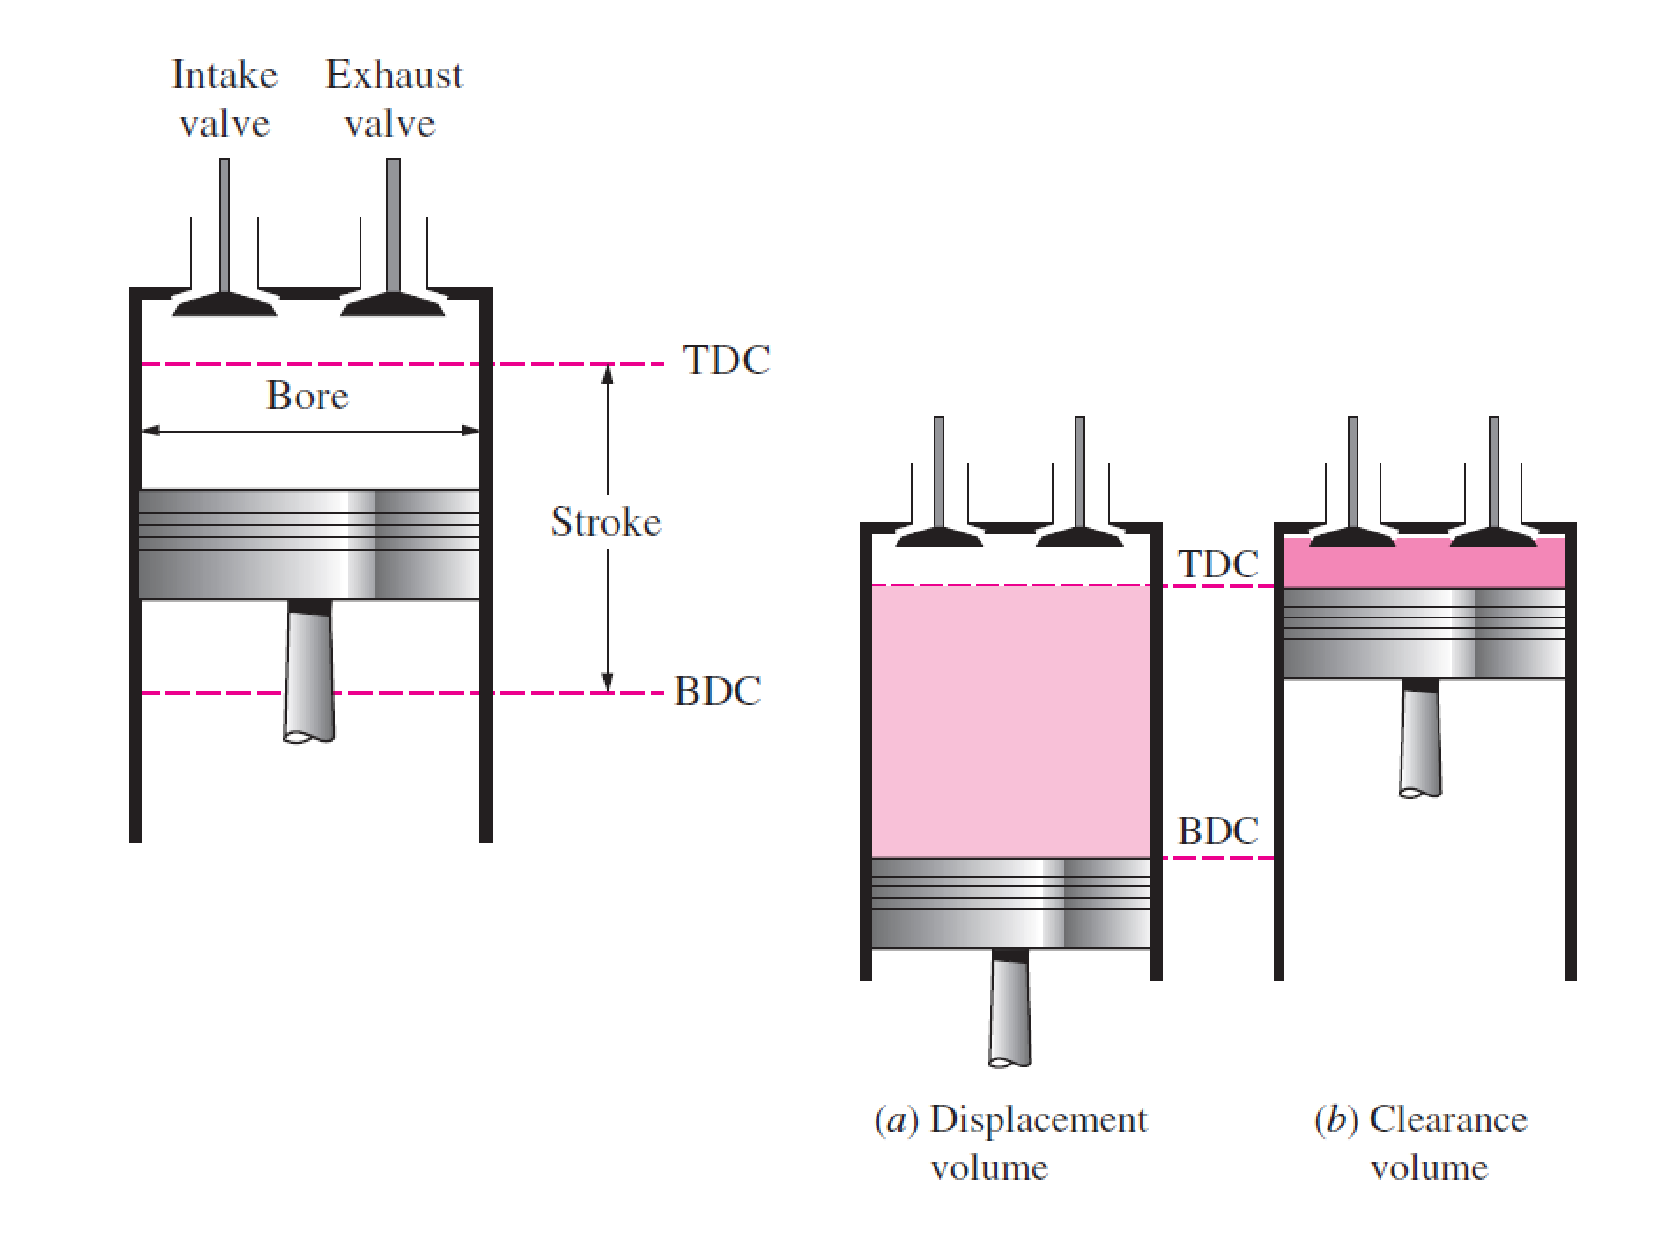
\includegraphics[width=7.5cm,clip]{./Pics/GasCycle_ReciprocatingEngine}
    \end{center}
   \end{figure}  
  \end{column}  
 \end{columns}
\end{frame}

%%%
%%% Slide
%%%
\begin{frame}
 \frametitle{Nomenclature}
   \begin{itemize}
    \item <1-> The \textcolor{blue}{mean effective pressure of the cycle ({\it MEP})} is a fictitious pressure that, if it acted on the piston during the entire power stroke, would \textcolor{blue}{produce the same amount of net work as that produced during the actual cycle}:
        \begin{displaymath}
          W_{\text{net}} =MEP \times \text{Piston area} \times \text{Stroke} \; \Longrightarrow \; MEP= \displaystyle\frac{W_{\text{net}}}{V_{\text{max}}-V_{\text{min}}}
        \end{displaymath}
    \item <2-> MEP is used as a parameter to compare performances of reciprocating engines of equal size:  Larger MEP $\Longrightarrow$ larger $W_{\text{net}}$
    \item <3-> Reciprocating engines are classified as:
     \begin{enumerate}
      \item <4->  \textcolor{blue}{{\it Spark-Ignition (SI)} Engines:} the combustion of the air–-fuel mixture is initiated by a spark plug (the mixture is at {\it flash point} conditions);
      \item <5->  \textcolor{blue}{{\it Compression-Ignition (CI)} Engines:} the air–-fuel mixture is self-ignited as a result of compressing the mixture above its self-ignition temperature.
     \end{enumerate}
   \end{itemize}
\end{frame}



\subsection{Ideal Carnot Cycle}
%%%
%%% Slide
%%%
\begin{frame}
 \frametitle{Carnot Cycle}
  \textcolor{blue}{Carnot cycle} has the highest possible efficiency and, similarly from previous lectures, consists of four stages:
  \begin{enumerate}
   \item <1-> Isothermal expansion; 
   \item <2-> Adiabatic expansion;
   \item <3-> Isothermal compression;
   \item <4-> Adiabatic compression.
  \end{enumerate}
\end{frame}

%%%
%%% Slide
%%%
\begin{frame}
 \frametitle{Carnot Cycle}
 \begin{columns}
  \begin{column}[c]{0.4\linewidth}
   \begin{itemize}
    \item <1-> A cylinder made with a $\lq$perfect' non-conducting material;
    \item <2-> A source of heat $\lq$H provides unlimited quantity of heat -- $T_{1}$;
    \item <3-> A material $\lq$S' with infinite heat capacity as so as its temperature remains constant $\left(T_{2}\right)$ irrespective of how much heat is supplied;
    \item <4-> Non-conducting cover $\lq$C'
   \end{itemize}
  \end{column}
  \begin{column}[c]{0.6\linewidth}
   \begin{figure}%
    \begin{center}
     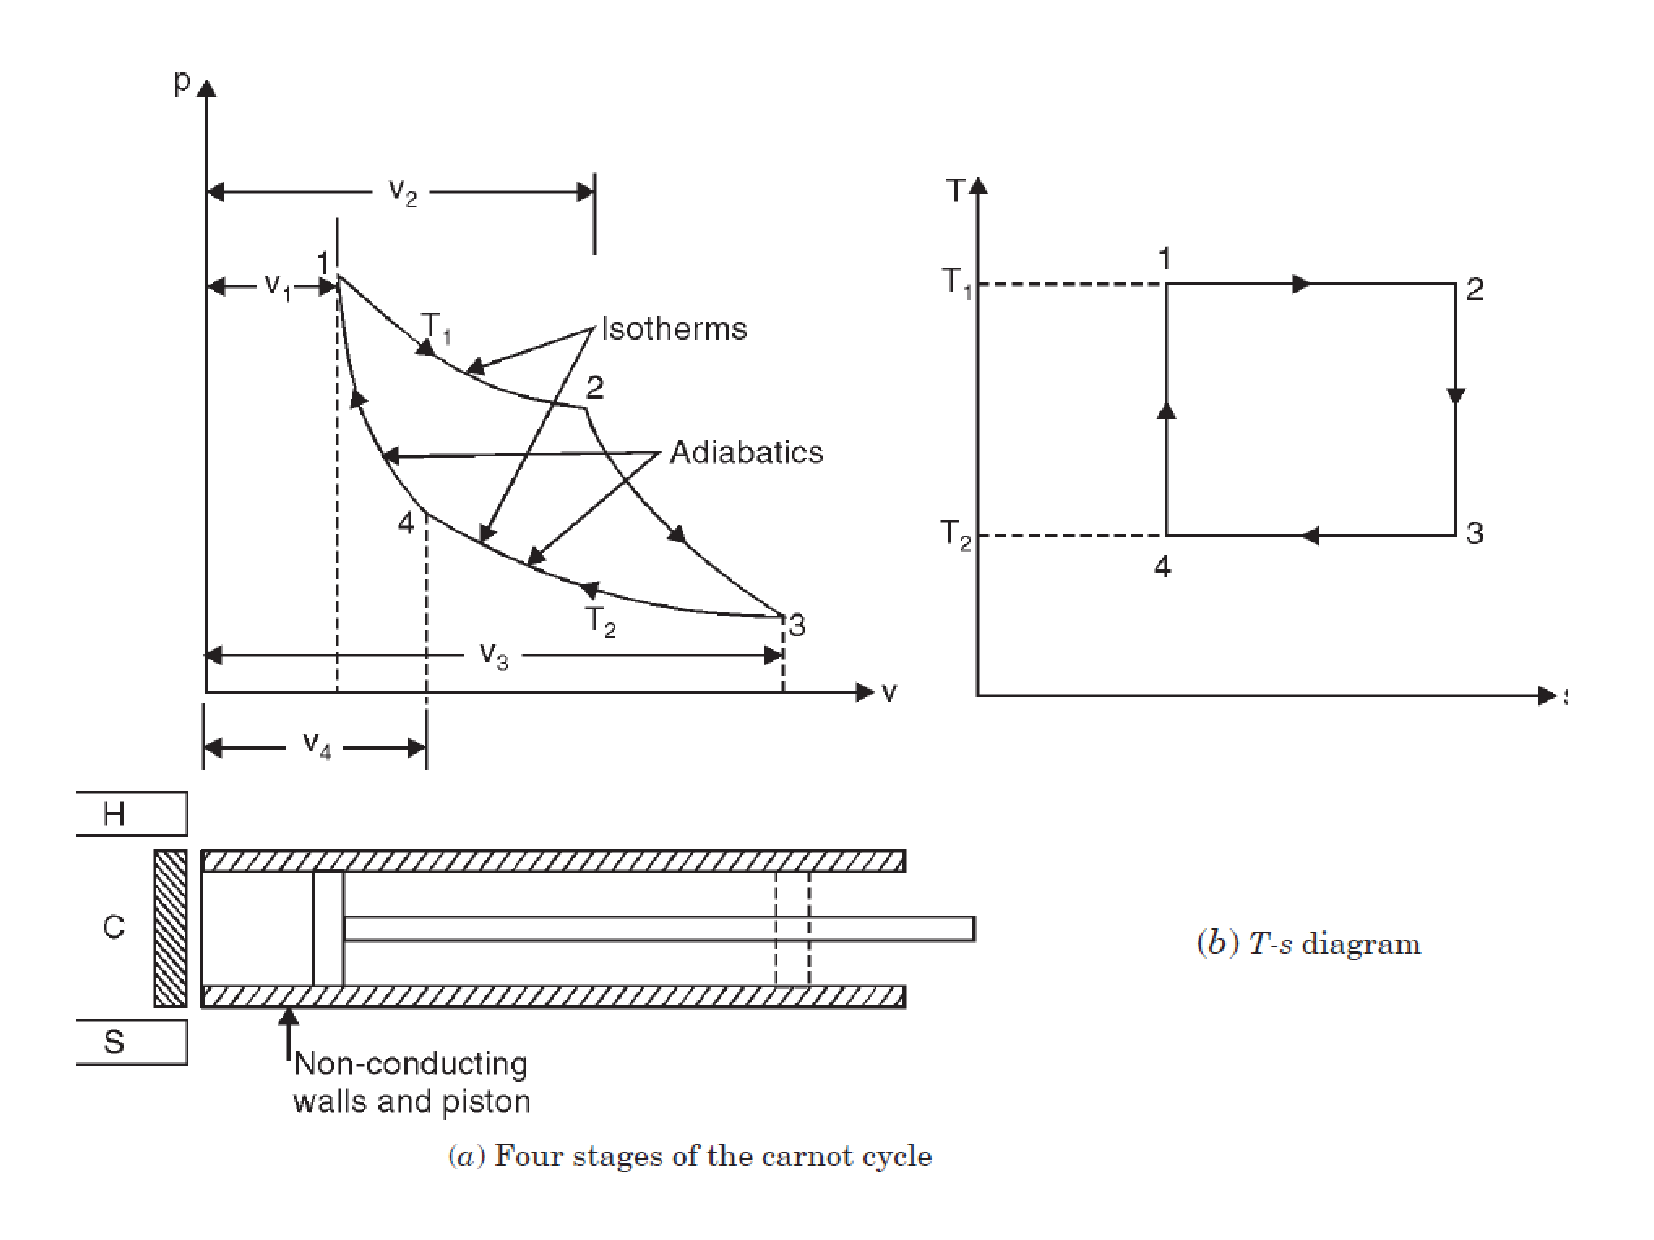
\includegraphics[width=7.5cm,clip]{./Pics/GasCycle_CarnotCycle}
    \end{center}
   \end{figure}  
  \end{column}  
 \end{columns}
\end{frame}

%%%
%%% Slide
%%%
\begin{frame}
 \frametitle{Carnot Cycle}
 \begin{columns}
  \begin{column}[c]{0.4\linewidth}
   \begin{itemize}
    \item <1-> \textcolor{blue}{1-2}: isothermal expansion $\left(T_{1}\right)$ due to heat $H$ been applied to the end of the cylinder. Heat supplied is $RT_{1}\ln r$, where $r$ is the ratio of expansion;
    \item <2-> \textcolor{blue}{2-3}: application of non-conducting cover to the end of the cylinder. This is followed by the adiabatic expansion and the temperature falls from $T_{1}$ to $T_{2}$;
   \end{itemize}
  \end{column}
  \begin{column}[c]{0.6\linewidth}
   \begin{figure}%
    \begin{center}
     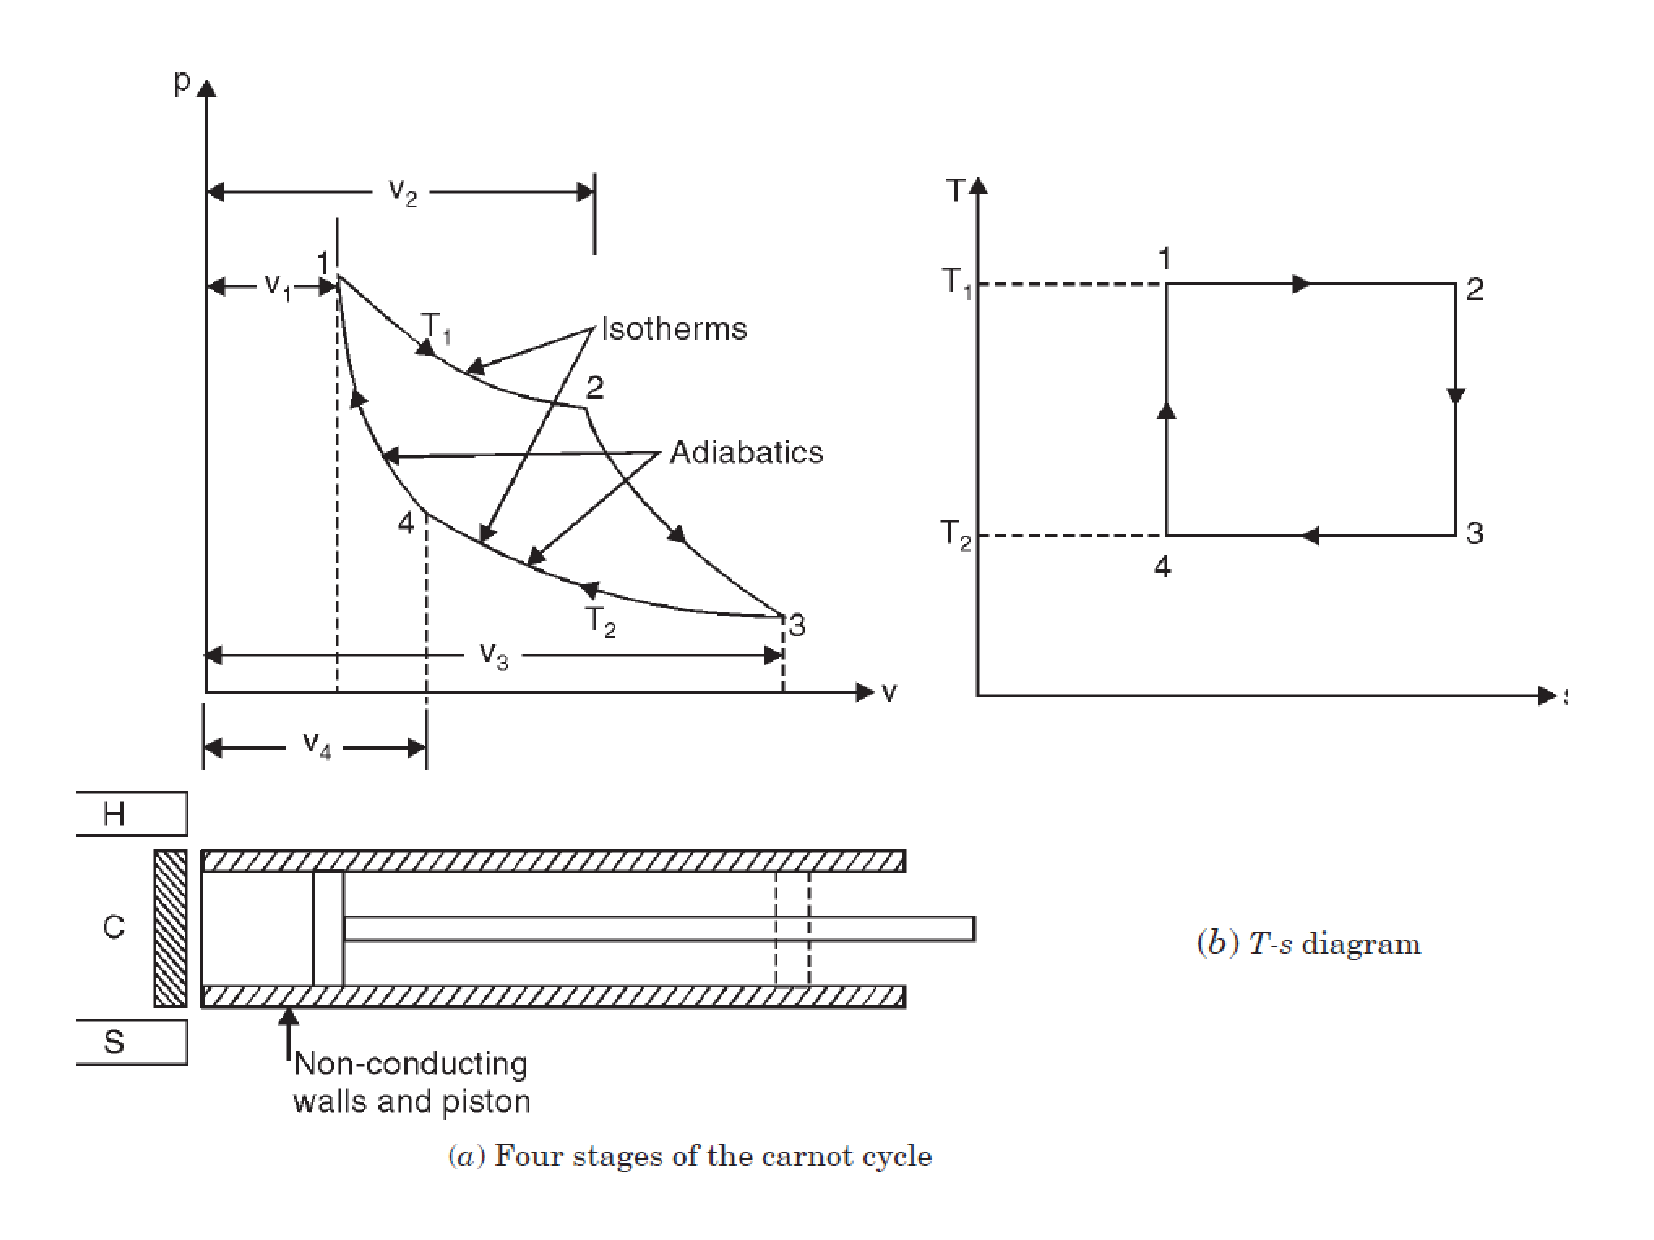
\includegraphics[width=7.5cm,clip]{./Pics/GasCycle_CarnotCycle}
    \end{center}
   \end{figure}  
  \end{column}  
 \end{columns}
\end{frame}

%%%
%%% Slide
%%%
\begin{frame}
 \frametitle{Carnot Cycle}
 \begin{columns}
  \begin{column}[c]{0.4\linewidth}
   \begin{itemize}
    \item <1-> \textcolor{blue}{3-4}: isothermal compression ($S$ is applied to the end of cylinder). Heat is rejected during this operation $\left(=RT_{2}\ln r\right)$;
    \item <2-> \textcolor{blue}{4-1}: repeated application of non-conducting cover and adiabatic compression due to temperature increase from $T_{2}$ to $T_{1}$.
   \end{itemize}
  \end{column}
  \begin{column}[c]{0.6\linewidth}
   \begin{figure}%
    \begin{center}
     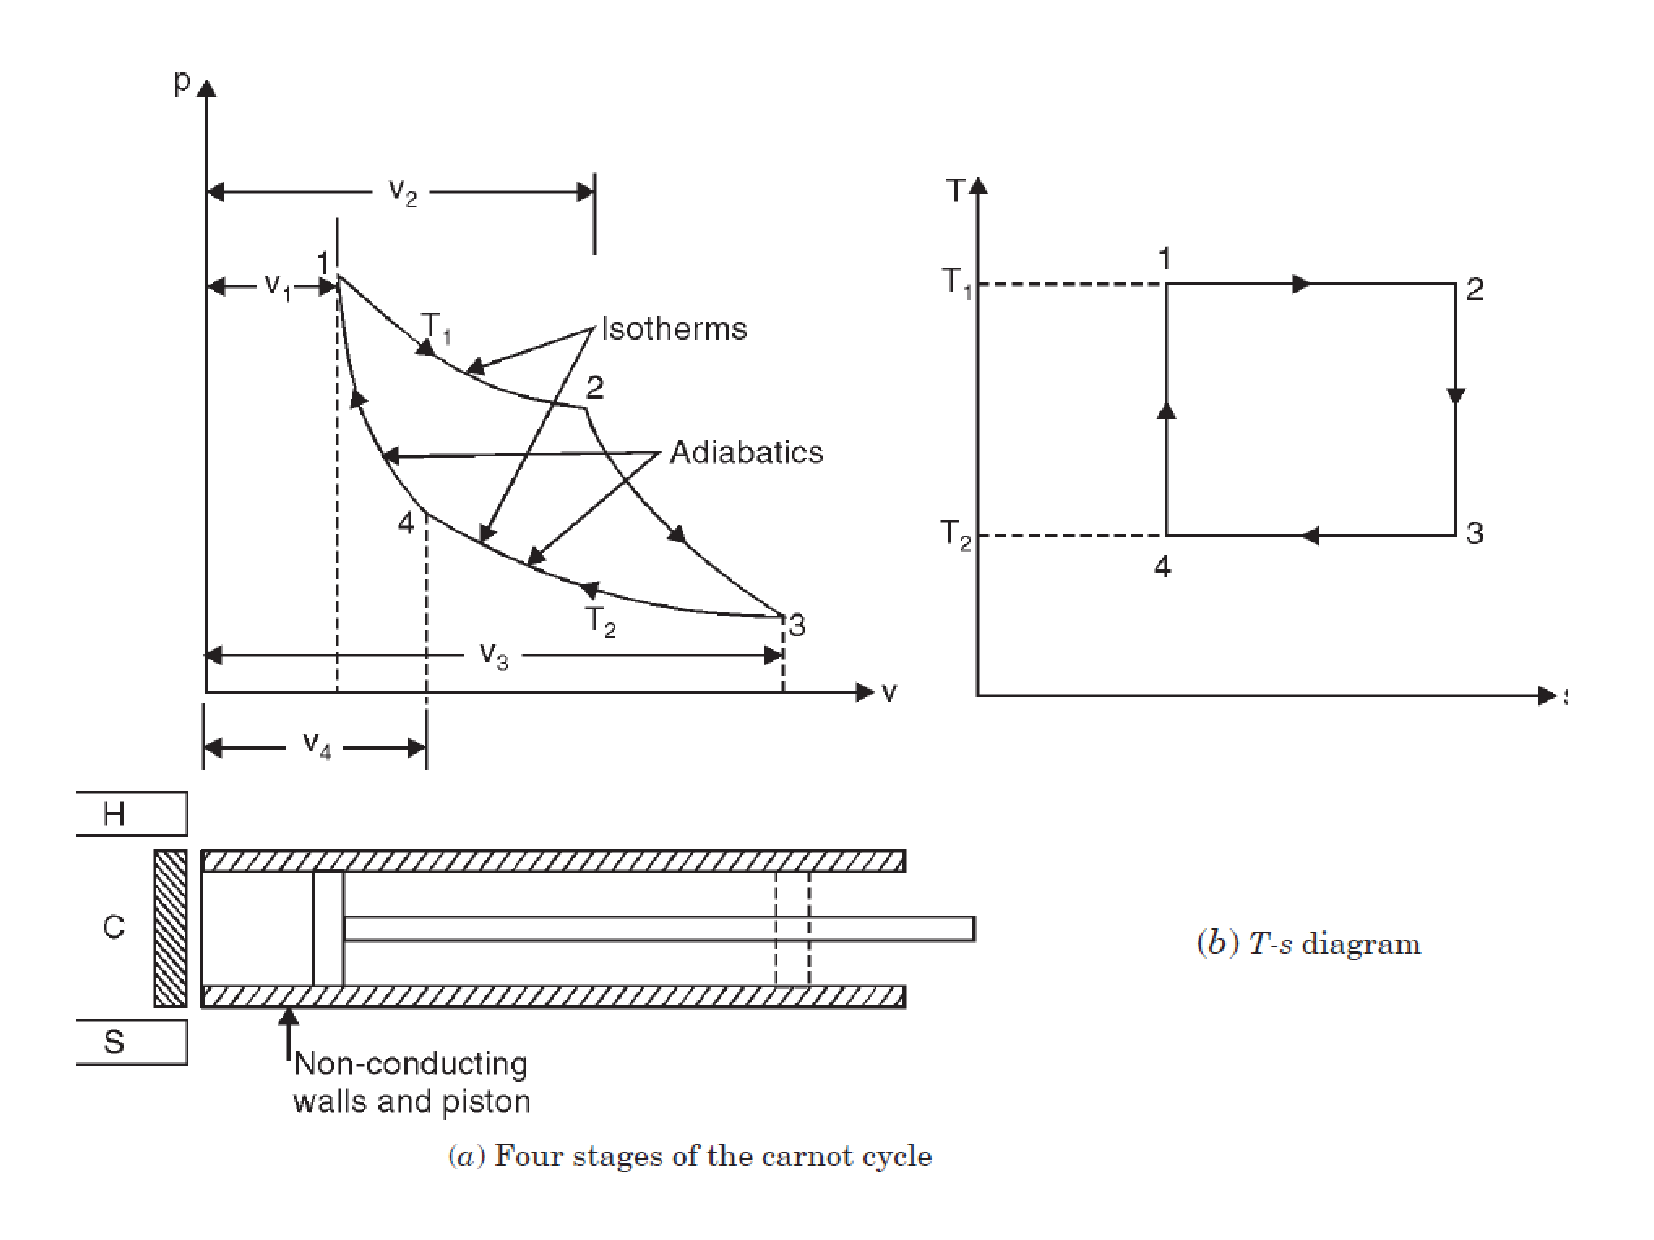
\includegraphics[width=7.5cm,clip]{./Pics/GasCycle_CarnotCycle}
    \end{center}
   \end{figure}  
  \end{column}  
 \end{columns}
\end{frame}



%%%
%%% Slide
%%%
\begin{frame}
 \frametitle{Carnot Cycle}
   \begin{itemize}
    \item <1-> The efficiency of the cycle is then given by
       \begin{eqnarray}
        \textcolor{blue}{\eta_{\text{Carnot}}} &=& \displaystyle\frac{\text{work done}}{\text{heat supplied}} = \displaystyle\frac{\text{heat supplied}-\text{heat rejected}}{\text{heat supplied}} \nonumber \\
                         &=& \displaystyle\frac{Q_{s}-Q_{r}}{Q_{s}}= \displaystyle\frac{R\left(T_{1}-T_{2}\right)\ln r}{RT_{1}\ln r} \nonumber  \\
                         &=& \displaystyle\frac{T_{1}-T_{2}}{T_{1}}\nonumber
       \end{eqnarray}
   \end{itemize}
\end{frame}




%%%
%%% Slide
%%%
\begin{frame}
 \frametitle{Carnot Cycle}
 \begin{columns}
  \begin{column}[c]{0.4\linewidth}
   \begin{itemize}
    \item <1-> $\textcolor{blue}{\eta_{\text{Carnot}}=\displaystyle\frac{T_{1}-T_{2}}{T_{1}}}$
    \item <1-> From the expression above, \textcolor{red}{the efficiency of the cycle can be readily enhanced if the $T_{2}$ decreases}. 
    \item <2-> In fact if $T_{2}\to 0$ (absolute zero temperature) $\Longrightarrow$ $\eta_{\text{Carnot}} \to 1$, i.e., 
    \item <3-> The efficiency reaches the maximum of \textcolor{blue}{100$\%$};
   \end{itemize}
  \end{column}
  \begin{column}[c]{0.6\linewidth}
   \begin{figure}%
    \begin{center}
     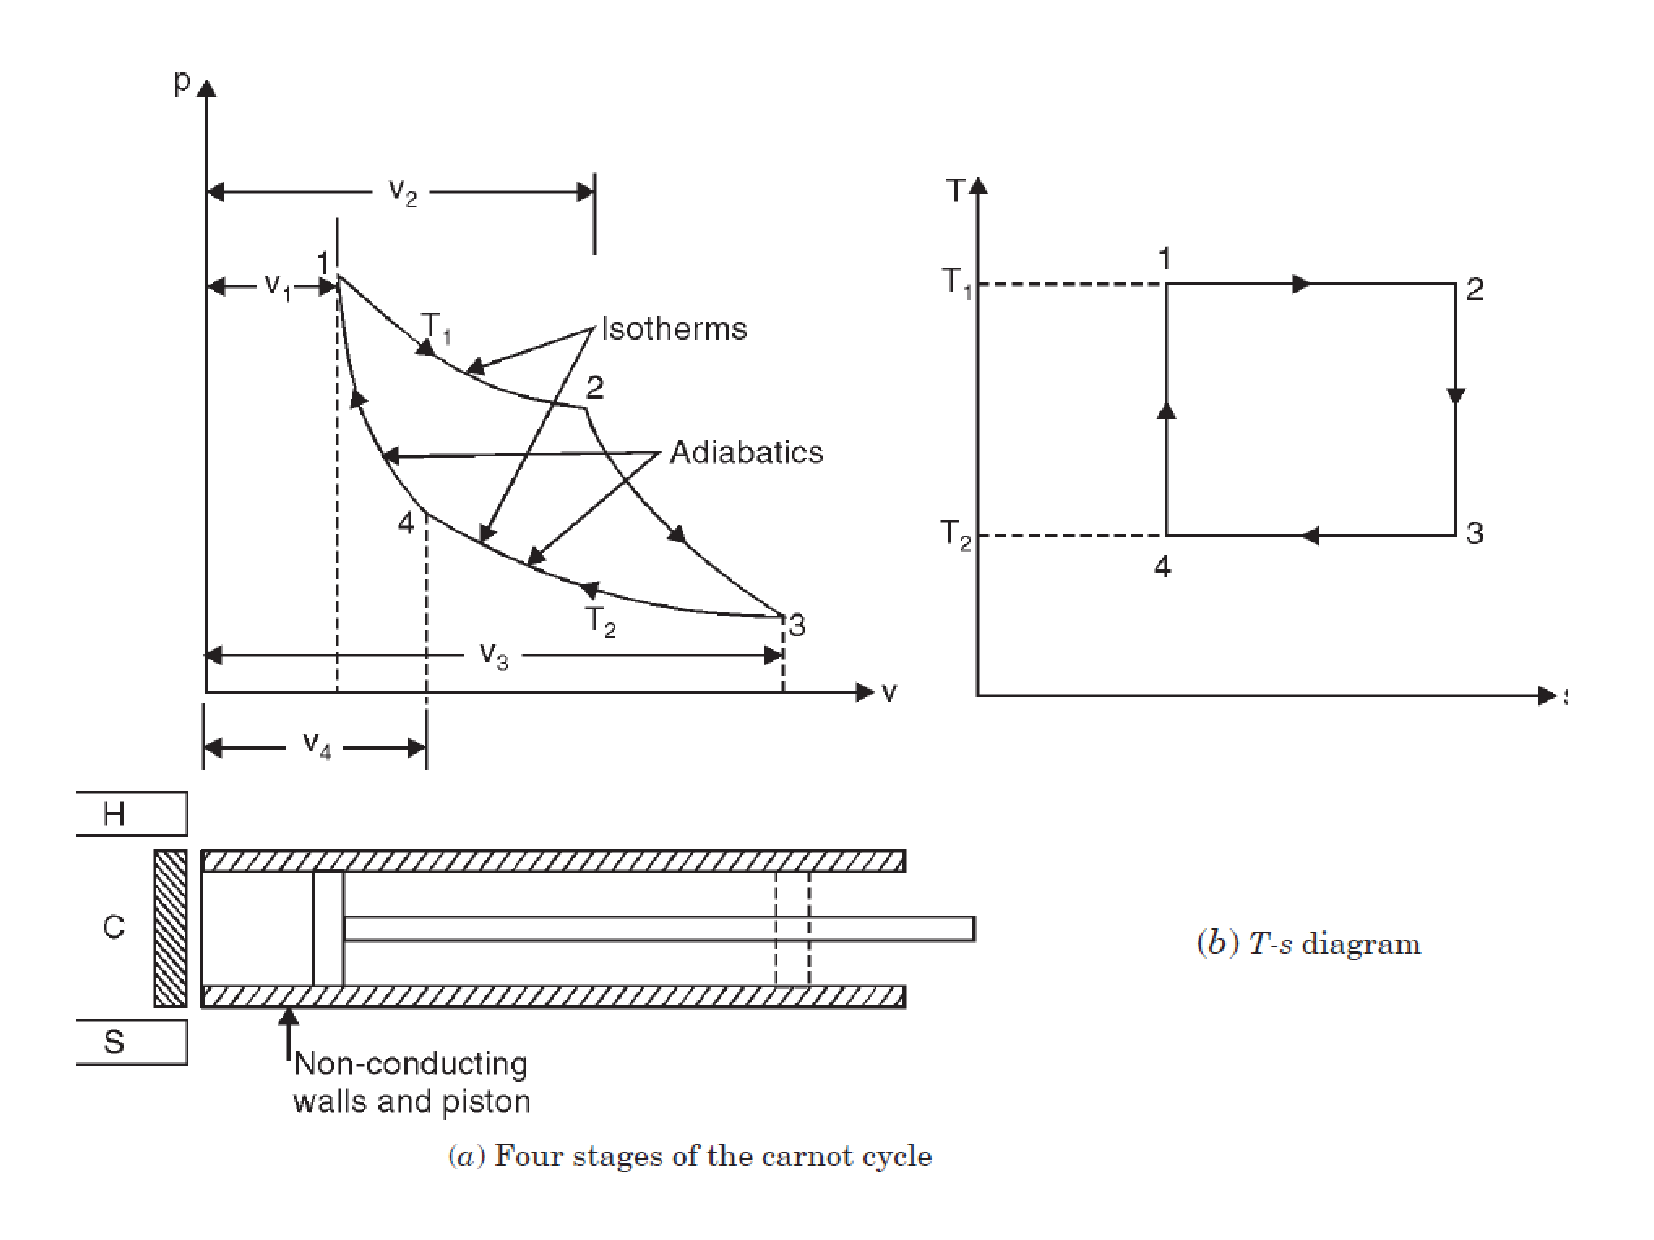
\includegraphics[width=7.5cm,clip]{./Pics/GasCycle_CarnotCycle}
    \end{center}
   \end{figure}  
  \end{column}  
 \end{columns}
\end{frame}

%%%
%%% Slide
%%%
\begin{frame}
 \frametitle{Carnot Cycle}
 \begin{columns}
  \begin{column}[c]{0.4\linewidth}
   \begin{itemize}
    \item <1-> In addition, we can not produce an engine that works on an ideal Carnot cycle as the piston would need to move:
     \begin{enumerate}
      \item <2-> very slow in the isothermal expansion ($\lq$forward stroke') and;
      \item <3-> very fast during the remainder of the adiabatic expansion $\Longrightarrow$ cycle is unfeasible.
     \end{enumerate}
   \end{itemize}
  \end{column}
  \begin{column}[c]{0.6\linewidth}
   \begin{figure}%
    \begin{center}
     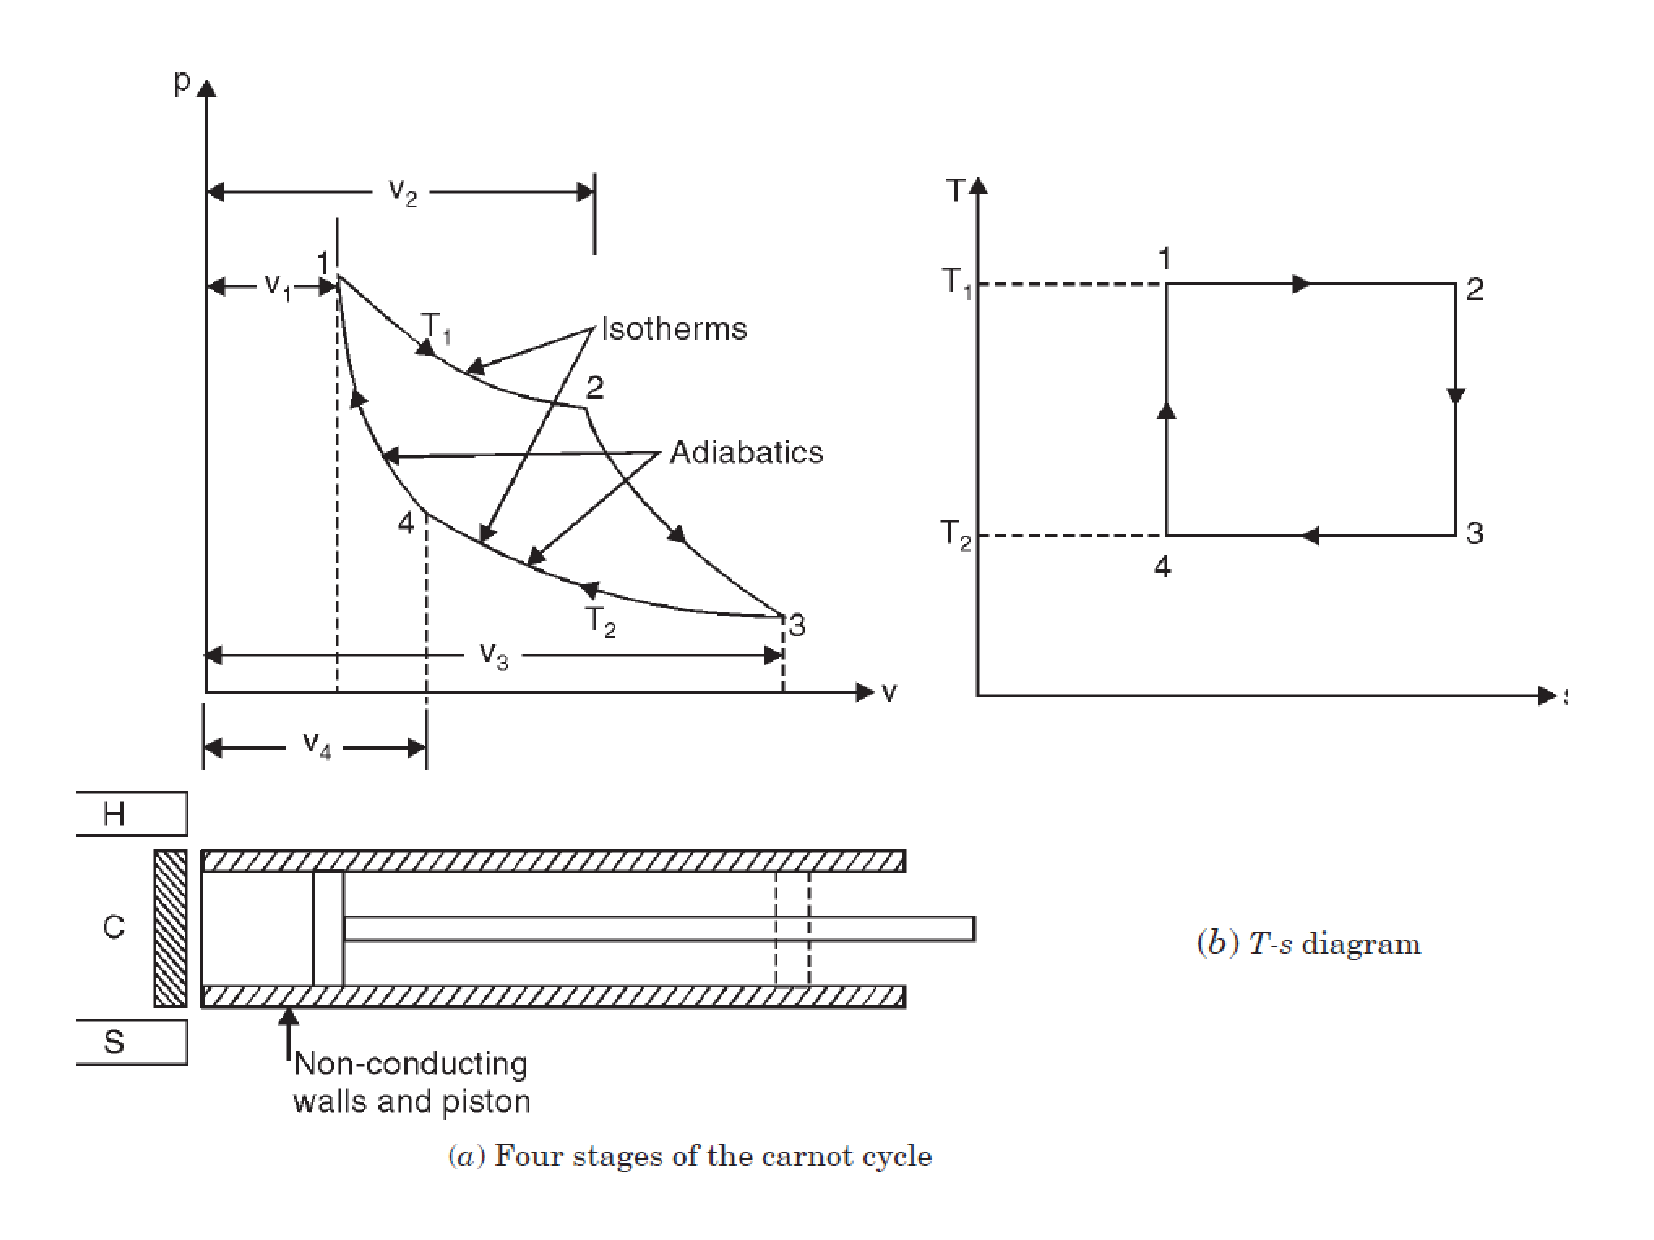
\includegraphics[width=7.5cm,clip]{./Pics/GasCycle_CarnotCycle}
    \end{center}
   \end{figure}  
  \end{column}  
 \end{columns}
\end{frame}


%%%
%%% Slide
%%%
\begin{frame}
 \frametitle{Carnot Cycle -- Example}
\textcolor{blue}{{\it In a Carnot cycle, the maximum pressure and temperature are limited to 18 bar and 410$^{o}$C. The ratio of isentropic compression is 6 and isothermal expansion is 1.5. Assuming the volume of the air at the beginning of isothermal expansion is 0.18 m$^{3}$, determine: (a) the temperature and pressures at all stages of the cycle; (b) change in entropy during isothermal expansion; (c) mean thermal efficiency of the cycle; (d) mean effective pressure (MEP) of the cycle and (e) theoretical power if there are 210 working cycles per minute.}}

\end{frame}


%%%
%%% Slide
%%%
\begin{frame}
 \frametitle{Carnot Cycle -- Example}
  \begin{columns}
   \begin{column}[c]{0.4\linewidth}
    \begin{itemize}
     \item Maximum pressure: $P_{1}=18$ bar;
     \item Maximum temperature: $T_{1}=T_{2}=410^{o}\text{C}=683.15\text{ K}$;
     \item Ratio of isentropic (or adiabatic) compression: $V_{4}/V_{1}=6$;
     \item Ratio of isothermal expansion: $V_{2}/V_{1}=1.5$;
     \item Volume of the air at the beginning of the isothermal expansion: $V_{1}=0.18\;m^{3}$.
    \end{itemize}
    \end{column}
    \begin{column}[c]{0.6\linewidth}
     \begin{figure}%
      \begin{center}
     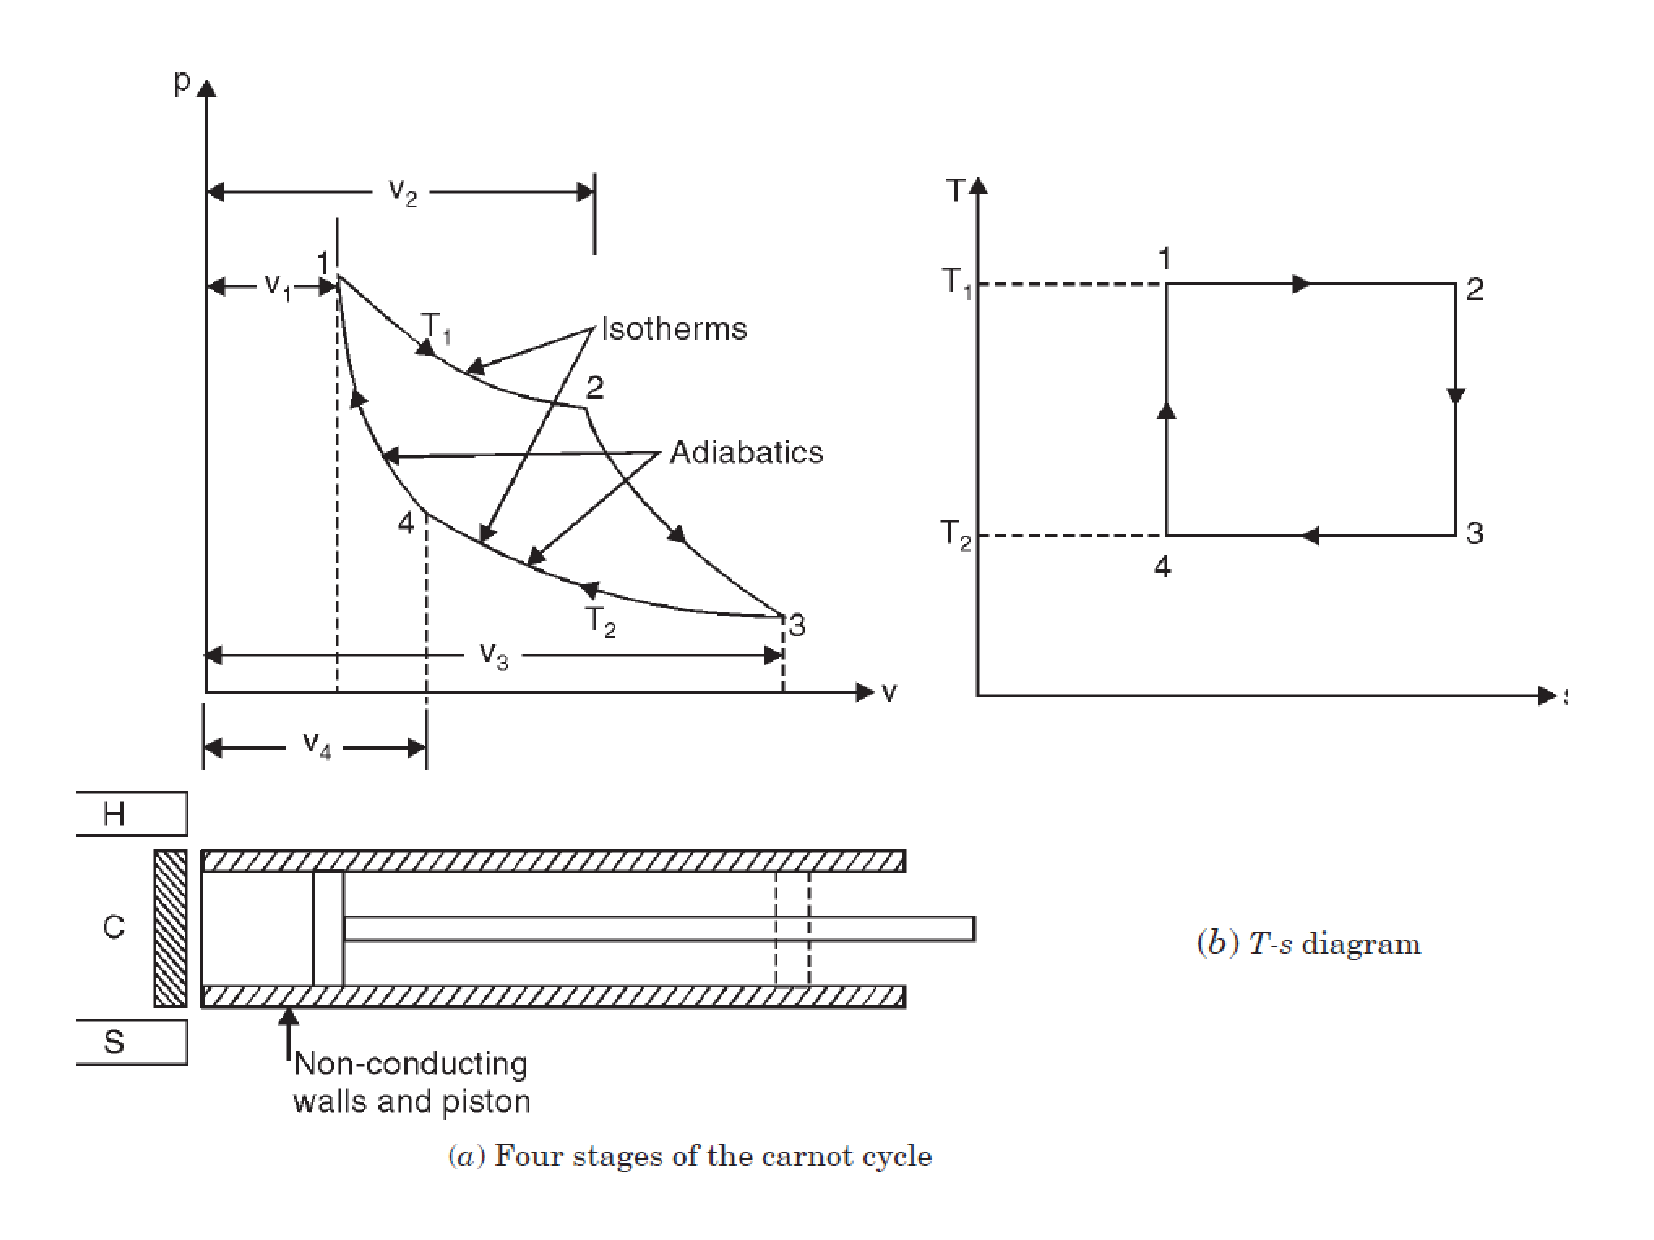
\includegraphics[width=7.5cm,clip]{./Pics/GasCycle_CarnotCycle}
    \end{center}
   \end{figure}  
  \end{column}  
 \end{columns}
\end{frame}



%%%
%%% Slide
%%%
\begin{frame}
 \frametitle{Carnot Cycle -- Example}
  \begin{columns}
   \begin{column}[c]{0.4\linewidth}
    Calculating $T_{i}$ and $P_{i}$:
    \begin{itemize}
     \item <2-> isentropic compression 4-1 (with $\gamma$ = 1.4):
      \begin{eqnarray}
       && \displaystyle\frac{T_{1}}{T_{4}}=\left(\displaystyle\frac{V_{4}}{V_{1}}\right)^{\gamma-1} \nonumber \\
       && T_{4}=333.2\text{ K } = T_{3} \nonumber \\
       && \displaystyle\frac{P_{1}}{P_{4}}=\left(\displaystyle\frac{V_{4}}{V_{1}}\right)^{\gamma} \nonumber \\
       && P_{4}=1.46\text{ bar }\nonumber
      \end{eqnarray}
     \item <3-> isothermal expansion 1-2:
      \begin{eqnarray}
       && P_{1}V_{1}=P_{2}V_{2} \nonumber \\
       && P_{2}=12\text{ bar} \nonumber
      \end{eqnarray}
    \end{itemize}
    \end{column}
    \begin{column}[c]{0.6\linewidth}
     \begin{figure}%
      \begin{center}
     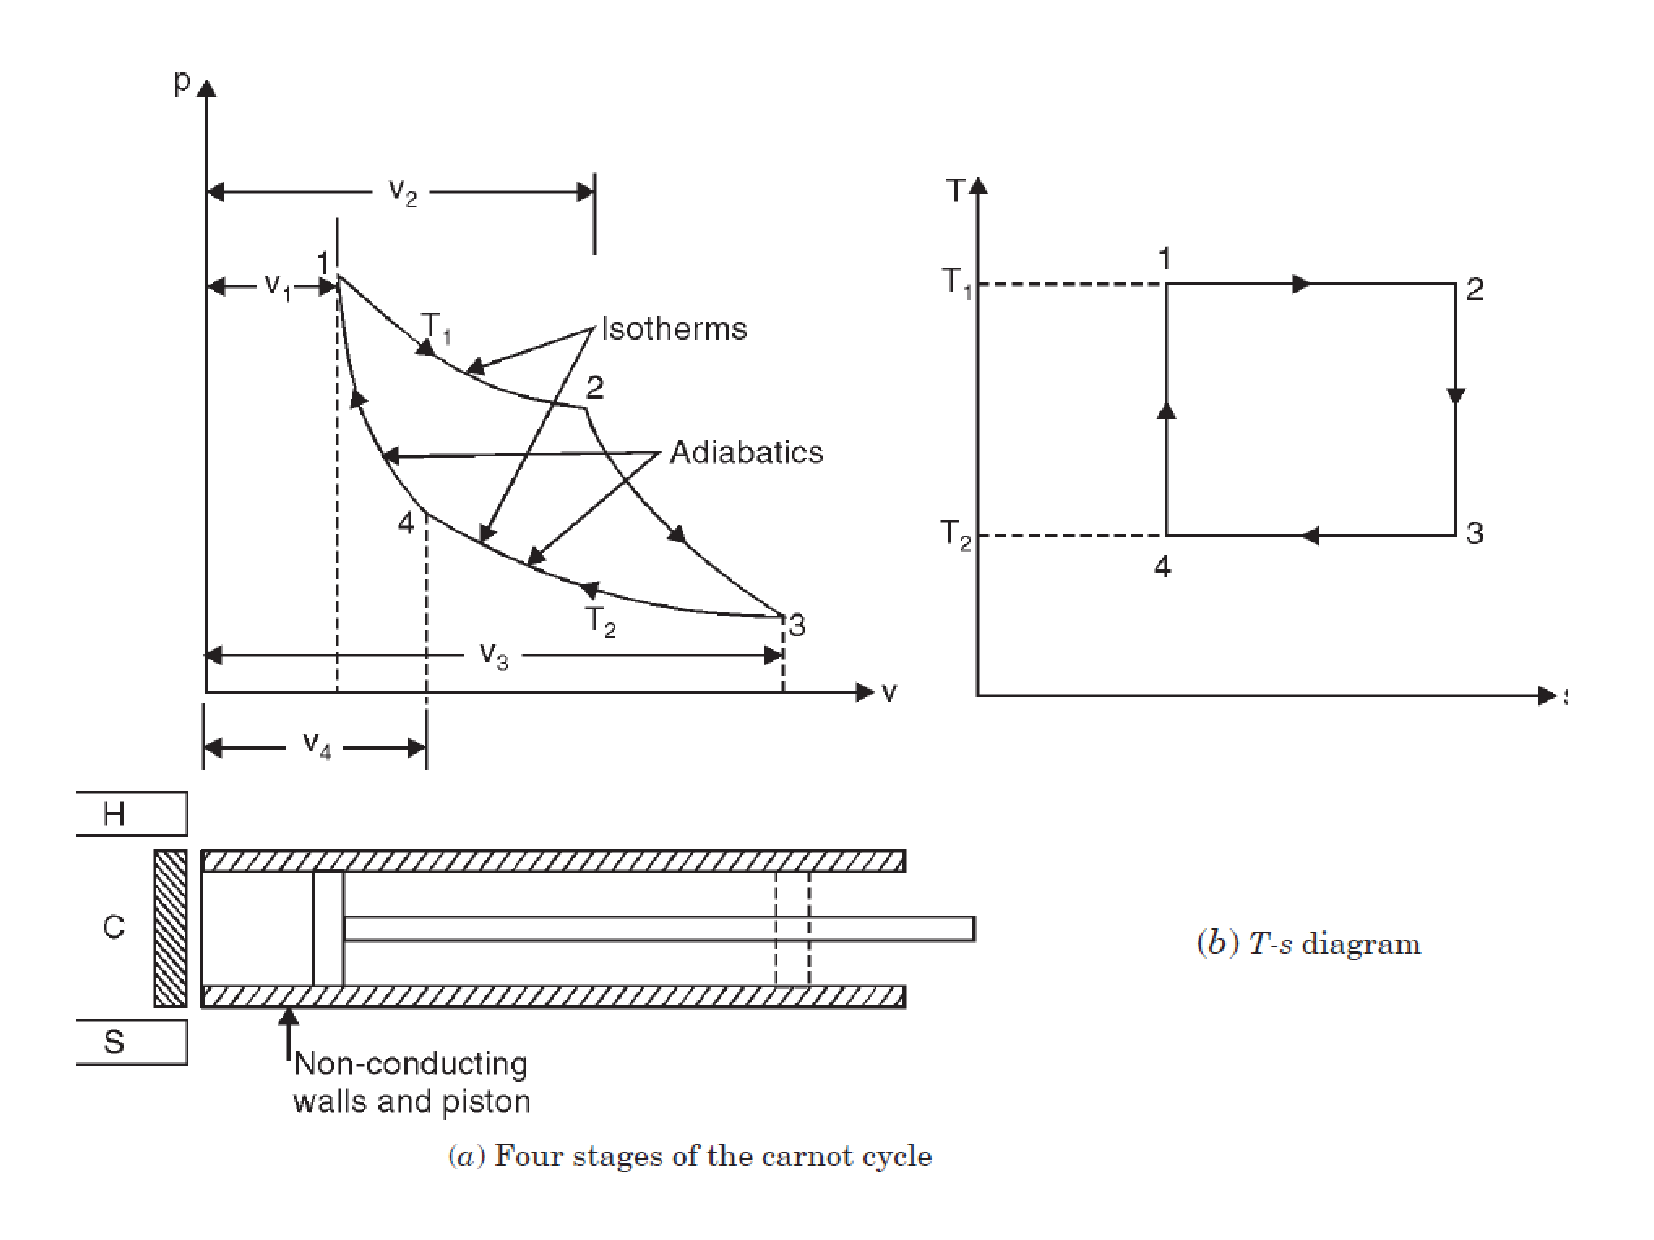
\includegraphics[width=7.5cm,clip]{./Pics/GasCycle_CarnotCycle}
    \end{center}
   \end{figure}  
  \end{column}  
 \end{columns}
\end{frame}


%%%
%%% Slide
%%%
\begin{frame}
 \frametitle{Carnot Cycle -- Example}
  \begin{columns}
   \begin{column}[c]{0.4\linewidth}
    \begin{itemize}
     \item <1-> isentropic expansion 2-3:
      \begin{eqnarray}
       && P_{2}V_{2}^{\gamma}=P_{3}V_{3}^{\gamma}\nonumber \\
       && \text{with } V_{4}/V_{1} = V_{3}/V_{2}\nonumber \\
       && P_{3}=0.97\text{ bar}\nonumber
      \end{eqnarray}
     \item <2-> Now that we calculated all $P_{i}$ and $T_{i}$, the variation of entropy during the isothermal expansion (1-2) is
       \begin{eqnarray}
         S_{2}-S_{1} &=& mR\ln\left(\displaystyle\frac{V_{2}}{V_{1}}\right)\nonumber \\
                     &=& \displaystyle\frac{P_{1}V_{1}}{T_{1}}\ln\left(\displaystyle\frac{V_{2}}{V_{1}}\right) \nonumber \\
                     &=& 0.192\text{ kJ/K} \nonumber
       \end{eqnarray}
    
       
    \end{itemize}
    \end{column}
    \begin{column}[c]{0.6\linewidth}
     \begin{figure}%
      \begin{center}
     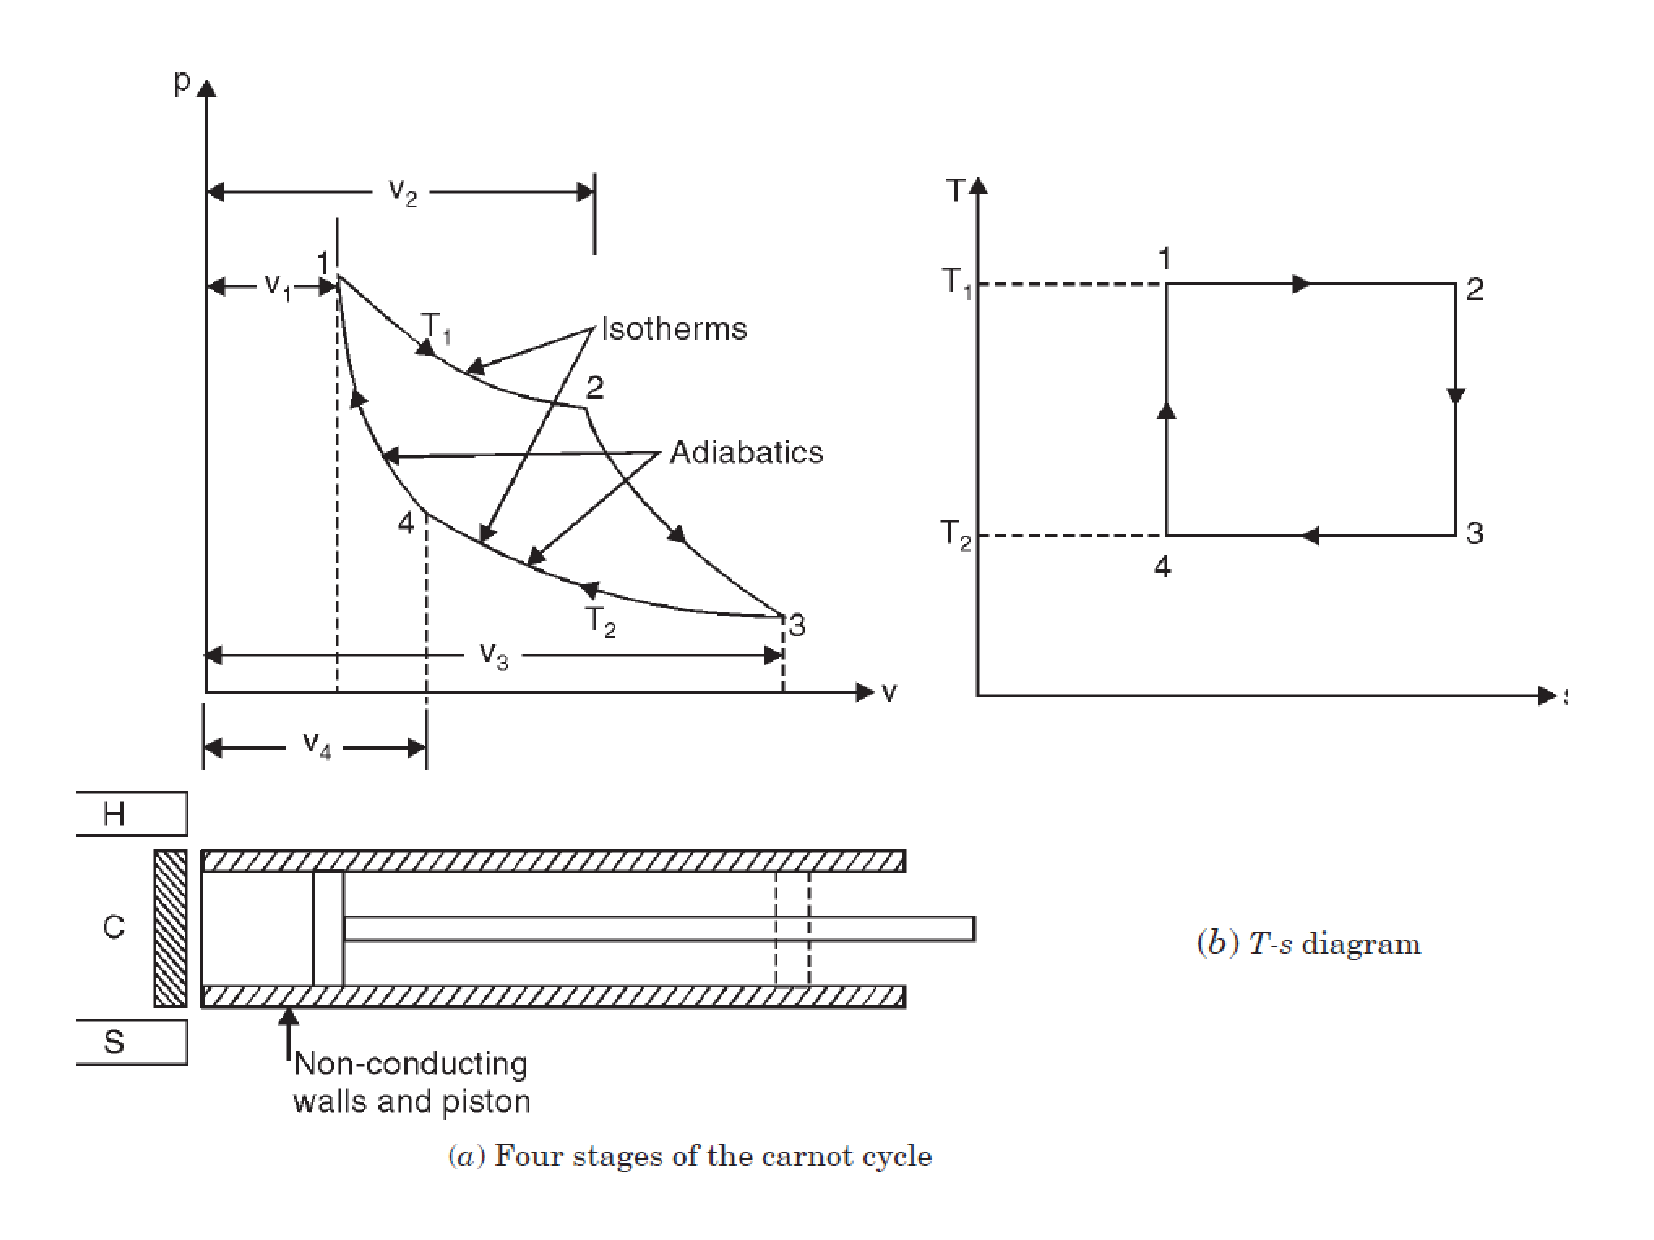
\includegraphics[width=7.5cm,clip]{./Pics/GasCycle_CarnotCycle}
    \end{center}
   \end{figure}  
  \end{column}  
 \end{columns}
\end{frame}

%%%
%%% Slide
%%%
\begin{frame}
 \frametitle{Carnot Cycle -- Example}
    \begin{itemize}
     \item <1-> The heat supplied to the system is:
      \begin{eqnarray}
         Q_{s}&=&P_{1}V_{1}\ln\left(\displaystyle\frac{V_{2}}{V_{1}}\right) = T_{1}\left(S_{2}-S_{1}\right)\nonumber \\
              &=&131.1\text{ kJ}\nonumber
      \end{eqnarray}

     \item <2-> The heat rejected by the system is:
      \begin{eqnarray}
         Q_{r}&=&P_{4}V_{4}\ln\left(\displaystyle\frac{V_{3}}{V_{4}}\right) = T_{4}\left(S_{3}-S_{4}\right) = T_{4}\left(S_{1}-S_{2}\right)\nonumber \\
             &=& 63.97\text{ kJ}\nonumber
      \end{eqnarray}
     \item <3-> And the efficiency:
       \begin{displaymath}
        \eta_{\text{Carnot}}=\displaystyle\frac{Q_{s}-Q_{r}}{Q_{s}}=0.512
       \end{displaymath}  
     
    \end{itemize}
\end{frame}


%%%
%%% Slide
%%%
\begin{frame}
 \frametitle{Carnot Cycle -- Example}
    \begin{itemize}
     \item <1-> The mean effective pressure of the cycle, {\it MEP}, (hypothetical pressure that acting upon the piston during the stroke will result on the same net work as the actual cycle) is given by
       \begin{displaymath}
         MEP=\displaystyle\frac{\text{work done}}{\text{stroke volume}}= \displaystyle\frac{Q_{s}-Q_{r}}{V_{s}}
       \end{displaymath}
     \item <2-> We need to calculate the volume of the stroke, $V_{s}=V_{3}-V_{1}$, and therefore $V_{3}$:
             \begin{eqnarray}
               \displaystyle\frac{V_{3}}{V_{1}}=\displaystyle\frac{V_{3}}{V_{2}}\displaystyle\frac{V_{2}}{V_{1}} \nonumber \\
               \text{but as } \displaystyle\frac{V_{3}}{V_{2}} = \displaystyle\frac{V_{4}}{V_{1}} \nonumber \\
               \displaystyle\frac{V_{3}}{V_{1}}=\displaystyle\frac{V_{4}}{V_{1}}\displaystyle\frac{V_{2}}{V_{1}}=6\times 1.5=9\nonumber \\
               \text{thus } V_{s}=V_{3}-V_{1}=9V_{1}-V_{1}=1.44\;m^{3}\nonumber
             \end{eqnarray}
     \item<3-> $P_{\text{me}}=0.466\text{ bar}$
     
    \end{itemize}
\end{frame}


%%%
%%% Slide
%%%
\begin{frame}
 \frametitle{Carnot Cycle -- Example}
    \begin{itemize}
     \item <1-> The power $\mathcal{P}$ of the engine is:
         \begin{displaymath}
           \mathcal{P}= \left(Q_{s}-Q_{r}\right) \mathcal{N}_{\text{cycles}}=\left(131.1-63.97\right)\displaystyle\frac{210}{60}=234.9\text{ kW}
         \end{displaymath}
     
    \end{itemize}
\end{frame}





\end{document}
